\chapter[INTERSCITY]{INTERSCITY}
\label{chapter:interscity}

O InterSCity é uma plataforma de cidades inteligentes nascida a partir de
estudos científicos que buscam abordar os principais desafios encontrados
no desenvolvimento de infraestruturas de cidades inteligentes \cite{nof2016}.
Está licenciado sob
MPLv2\footnote{\url{www.mozilla.org/en-US/MPL/2.0/}} (\textit{Mozilla Public License
Version 2.0}), foi construído com a
utilização da arquitetura MSA (\textit{Microservices Architecture}) e tem como principal
objetivo prover os serviços e integrações necessárias para a construção de
aplicações de cidades inteligentes complexas \cite{delesposte2017}. Baseando-se
no desenvolvimento colaborativo e na utilização de tecnologias software livre,
o projeto é desenvolvido com a ajuda de diversos colaboradores que, utilizando
práticas ágeis, atuam na manutenção e evolução da plataforma ao longo do tempo
\cite{delesposte2017}.

A maior parte dos microsserviços\footnote{Os termos microsserviços, módulos e
componentes serão utilizados intermitentemente, mas apresentando o mesmo
significado.} da plataforma foram escritos em Ruby on Rails
seguindo padrões que buscam extensibilidade e qualidade, e levando em conta
princípios\footnote{Os princípios seguidos pelo InterSCity são apresentados no
Apêndice \ref{appendix:principles}.} importantes na busca por uma melhor arquitetura.
A partir de experimentos feitos foi possível analisar
o estado atual da performance e da escalabilidade do InterSCity, que se mostrou
promissor \cite{delesposte2017}. O projeto encontra-se hospedado no
Gitlab\footnote{\url{https://gitlab.com/smart-city-software-platform}},
onde é possível ter acesso ao código fonte e documentação, bem como um exemplo de
cliente que ilustra o uso da plataforma.

\section{ARQUITETURA}
\label{sec:architecture}

O InterSCity segue uma arquitetura de microsserviços distribuída que
possibilita armazenamento, análise, processamento, composição e integração de
dados de recursos de cidades inteligentes \cite{delesposte2017}. Os
microsserviços são desacoplados entre si e se comunicam através de requisições REST
(\textit{Representational State Transfer}) e passagem de mensagem, modelo importante em
contextos de concorrência por conta do isolamento provido \cite{armstrong2003}.

\pagebreak
\begin{figure}[hbt]
  \centering
    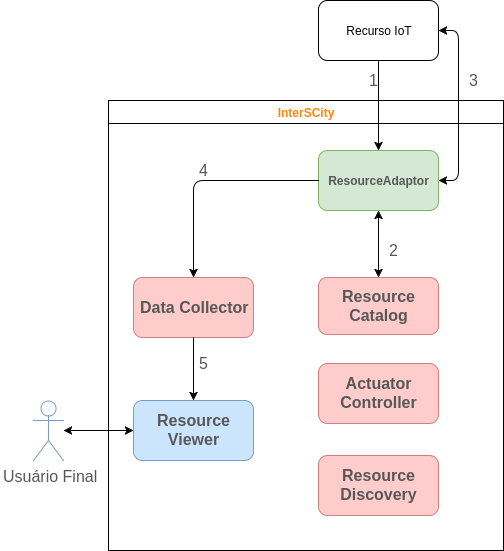
\includegraphics[scale=0.5]{figuras/interscity_flow.png}
  \caption{Ciclo de vida de um recurso IoT no InterSCity. Baseado em: \citeonline{delesposte2017}.}

  \label{fig:interscity-lifecycle}
\end{figure}

A Figura \ref{fig:interscity-lifecycle} ilustra o ciclo de vida típico de um
recurso IoT (\textit{Internet of Things}) na plataforma. Inicialmente um recurso IoT (1) faz um pedido de
registro na plataforma via Resource Adaptor, que (2) cadastra o recurso no
microsserviço Resource Catalog (3) e informa o UUID
(identificador único) que será utilizado internamente desse passo em diante.
Após, a comunicação entre o Resource Adaptor e o dispositivo IoT terá
continuidade, mas (4) os dados terão como destino o módulo Data Collector,
que armazenará as informações. Por fim, (5) as informações contidas no
Data Collector são disponibilizadas, podendo ser apresentadas para um usuário
final via Resource Viewer ou consumidas por uma aplicação cliente.

Os microsserviços do InterSCity têm responsabilidades atômicas e bem
definidas, princípio chave para que a plataforma contemple requisitos funcionais
e não-funcionais. O microsserviço \textbf{Resource Adaptor} é o grande
responsável pela comunicação entre os dispositivos IoT e a plataforma,
funcionando como um mediador durante as requisições \cite{delesposte2017}.

O \textbf{Data Collector} e o \textbf{Resource Catalog} tem papéis parecidos,
mas enquanto o primeiro gerencia e armazena dados históricos de medições dos
dispositivos, o segundo tem o papel de gerenciar e armazenar o registro dos
dispositivos na plataforma \cite{delesposte2017}.

\begin{figure}[hbt]
  \centering
    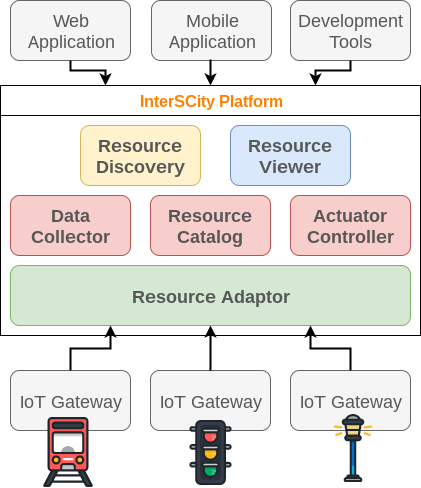
\includegraphics[scale=0.5]{figuras/interscity_architecture.png}
    \caption{Arquitetura do InterSCity. Fonte: \citeonline{delesposte2017}.}
  \label{fig:interscity-architecture}
\end{figure}


O \textbf{Resource Viewer} e o \textbf{Resource Discovery}, por outro lado,
são similares por manipularem e utilizarem o Data Collector e o Resource
Catalog em sua execução. O Resource Viewer tem como objetivo apresentar ao
usuário final os dados dos recursos, enquanto o Resource Discovery provê uma API
 de busca por dispositivos disponíveis, possibilitando o uso de filtros
\cite{delesposte2017}. Por fim, o \textbf{Actuator Controller} provê serviços
para requisições nos recursos IoT atuadores registrados na plataforma,
armazenando os dados e possibilitando auditoria \cite{delesposte2017}. A Figura
\ref{fig:interscity-architecture} trás uma visão geral da arquitetura com todos
os microsserviços reunidos, apresentando as fronteiras entre a plataforma,
as aplicações clientes e os dispositivos.

\section{GERÊNCIA DE CONFIGURAÇÃO E DEPENDÊNCIAS}

Outro aspecto que recebe atenção no desenvolvimento do InterSCity é a gerência
de configuração, que atualmente utiliza tecnologias que reduzem o esforço,
promovem o isolamento entre a plataforma e o ambiente hospedeiro
e aumentam a segurança no desenvolvimento. A gerência de configuração do
InterSCity é guiada por contêineres do
Docker\footnote{\url{https://www.docker.com/}}, onde cada microsserviço e
dependência externa são executados em contêineres separados. O desenvolvimento
da plataforma também faz extenso uso do
Git\footnote{\url{https://git-scm.com/}}, de modo que a configuração de um
ambiente de teste do InterSCity tenha como pré-requisitos somente esses
dois projetos: Docker e Git.

Cada microsserviço da plataforma contém seu próprio repositório, permitindo que
evoluam de maneira distribuída. Com o propósito de ajudar no desenvolvimento,
o InterSCity apresenta um repositório
principal\footnote{\url{https://gitlab.com/smart-city-software-platform/dev-env}},
que funciona como \textit{repositório mestre}, sendo os repositórios dos
microsserviços da plataforma submódulos.

\section{PROPOSTA E METODOLOGIA PARA IMPLEMENTAÇÃO DO SERVIÇO DE PROCESSAMENTO DE DADOS}

Atualmente a plataforma está em desenvolvimento, e embora não conte
com uma camada de processamento de dados ideal, certo esforço pela equipe do
InterSCity culminou em um serviço de processamento provisório, que pôde servir
de base para o desenvolvimento da proposta do novo serviço de processamento. Houve ainda a
troca de tecnologia de banco de dados no microsserviço Data Collector, que
passou do Postgres (tecnologia SQL) para o MongoDB (tecnologia NoSQL), troca
importante na busca por uma maior elasticidade no volume de dados. A equipe
do InterSCity nomeou a camada provisória de \textbf{Data Processor}, que
conta com uma configuração pronta para uso do Apache Spark e
\textit{scripts} que ilustram situações de uso dessa tecnologia. O Data
Processor, contudo, apresenta uma solução bem específica, não podendo ser
reaproveitado por outras aplicações.

Nesse contexto, neste trabalho, desenvolvemos um novo serviço de processamento de dados que
permite que aplicações de cidades inteligentes utilizem o InterSCity no processamento e
análise de seus dados. Através do novo serviço,
um maior volume de dados poderá ser processado pela plataforma, possibilitando
também o uso de algoritmos e operações complexas. O novo serviço
faz uso de um padrão de projeto de \textit{Big Data} adequado para o contexto
de cidades inteligentes e compatível com a arquitetura atual do InterSCity.
Fizemos um levantamento das arquiteturas de \textit{Big Data} candidatas, assim
como um estudo a respeito de possíveis ferramentas a serem utilizadas. Esse
levantamento teve restrições, como: somente projetos software livre
foram levados em conta e ferramentas que trouxessem grandes mudanças ao
ecossistema do InterSCity teriam pouca prioridade.

A nova arquitetura de processamento de dados, apresentada neste trabalho, visa
atender requisitos típicos de cidades inteligentes e possibilita a extensão
para trabalhos futuros. A nova arquitetura permite, por exemplo, que um
canal de dados possa ser utilizado, mesmo que faça uso de uma
maior massa de dados, ou que uma aplicação processe seus dados através de
operações específicas e customizadas, por chamadas diversas. 
Por fim, fornecemos um exemplo de aplicação que utiliza a arquitetura
desenvolvida, como prova de conceito.
